\begin{figure}[h]
    \centering
    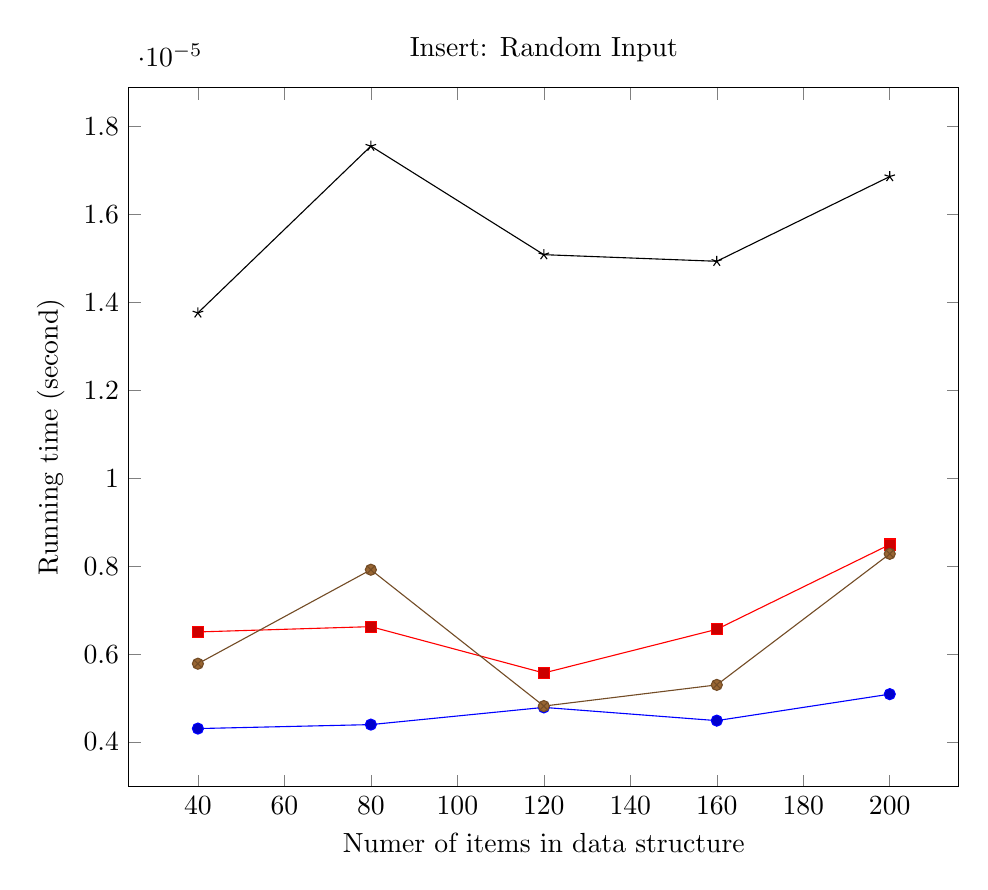
\begin{tikzpicture}
        \begin{axis}[
            xlabel={Numer of items in data structure},
            ylabel={Running time (second)},
            title={Insert: Random Input},
            width=\textwidth
        ]
		\addplot coordinates {
			(40, 4.306807315548889e-06)
			(80, 4.3971599165734674e-06)
			(120, 4.78868785435127e-06)
			(160, 4.487512517600823e-06)
			(200, 5.0898631911044935e-06)
		};
		\addplot coordinates {
			(40, 6.505387273836316e-06)
			(80, 6.625857408536218e-06)
			(120, 5.571743729905488e-06)
			(160, 6.5656223411841855e-06)
			(200, 8.493144496396488e-06)
		};
		\addplot coordinates {
			(40, 5.782566465631356e-06)
			(80, 7.920911356570914e-06)
			(120, 4.818805388026593e-06)
			(160, 5.300685926828974e-06)
			(200, 8.282321760672007e-06)
		};
		\addplot coordinates {
			(40, 1.3763712889552915e-05)
			(80, 1.75585221326241e-05)
			(120, 1.5088884371258771e-05)
			(160, 1.4938296702884934e-05)
			(200, 1.6865818858094462e-05)
		};
        \legend{}
        \end{axis}
    \end{tikzpicture}
    \caption{Average of 0 operations, benchmarked every 0, starting at 0.}
\end{figure}